\documentclass[12pt]{article}
\usepackage[utf8]{inputenc}
\usepackage{graphics}
\usepackage{graphicx}
\usepackage{float}
\usepackage{eso-pic}
\usepackage[top=3cm,bottom=3cm,left=2.5cm,right=2.5cm,headsep=10pt,letterpaper]{geometry}
\usepackage{verbatim}
\usepackage{amssymb}
\usepackage{stmaryrd}
\usepackage{mathrsfs, amsmath}
\usepackage{listings}
\usepackage{indentfirst}
\usepackage{tabularx}
\usepackage{hyperref}
\lstset{language = MATLAB}
\usepackage{abstract}
\usepackage{amsmath}
\usepackage{amsthm}
\usepackage{tcolorbox}
\usepackage{enumitem}

\begin{document}

\newpage
\newpage
\newtheorem{theorem}{Theorem}

\begin{titlepage}

    \begin{center}
        \vspace*{2.5in}
            \huge
            \textbf{{Homework 1}}\\
            \large
            \textbf{Numerical Solutions to Partial Differential Equations}\\
    \end{center}
    ~\vfill
    \noindent \textsc{Colorado School of Mines}\\
    \textsc{Department of Applied Mathematics and Statistics}\\
    
    \vspace{1cm}
    \noindent \textsc{\textbf{AUTHOR INFORMATION}}\\
    \noindent Hugh Scribner\footnote{Computational and Applied Mathematics}\\ 
    \vspace{1mm}
    
\end{titlepage}

\newpage

\tableofcontents

\newpage

\newpage
\section{Problem 1}
 \begin{tcolorbox}
        \textbf{Problem Statement:}\\
        Simulate the stokes equations using a finite difference method on a staggered grid. Provide an image of the magnitude of the velocity vector.
    \end{tcolorbox}
    
    \textbf{Solution:}
        Below is a figure of the magitude of the velocity 
                \begin{figure}[H]
                    \begin{centering}
                        \centering
                            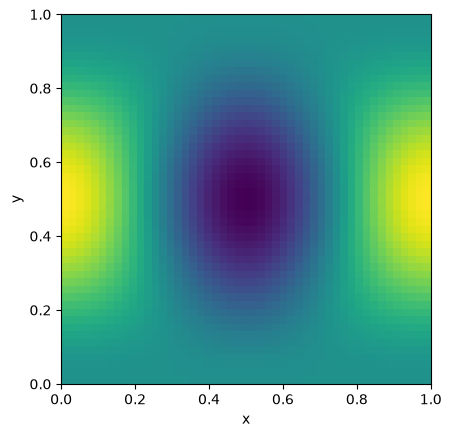
\includegraphics[scale=.75]{Images/mag_u.png}
                            \caption{Magnitude of fluid velocity, $\vec{u}$, as predicted by a finite difference stokes solver.}
                            \label{fig: u_magnitude}
                    \end{centering}
                \end{figure}
\newpage
\section{Problem 2}
 \begin{tcolorbox}
        \textbf{Problem Statement:}\\
        
    \end{tcolorbox}
    
    \textbf{Solution:}

\newpage
\section{Problem 3}
 \begin{tcolorbox}
        \textbf{Problem Statement:}\\
        
    \end{tcolorbox}
    
    \textbf{Solution:}
    
\end{document}
